\section{平面问题的基本理论}
\subsection{两类问题}
\begin{enumerate}
	\item 平面应力问题: 只在平面内有应力,与该面垂直方向的应力可忽略,例如薄板拉压问题。\[\underset{\text{独立}}{\underbrace{\sigma _x,\sigma _y,\tau _{xy},\varepsilon _x,\varepsilon _y,\gamma _{xy},u,v}}\underset{\text{非独立}}{\underbrace{\varepsilon _{z,}w}}\]
	\item 平面应变问题: 只在平面内有应变,与该面垂直方向的应变可忽略,例如水坝侧向水压问题。\[\underset{\text{独立}}{\underbrace{\sigma _x,\sigma _y,\tau _{xy},\varepsilon _x,\varepsilon _y,\gamma _{xy},u,v}}\underset{\text{非独立}}{\underbrace{\sigma _z}}\]
\end{enumerate}

\subsection{平衡方程}
\begin{equation}
	\begin{cases}
	\frac{\partial \sigma _x}{\partial x}+\frac{\partial \tau _{xy}}{\partial y}+f_x=0\\
	\frac{\partial \sigma _y}{\partial y}+\frac{\partial \tau _{xy}}{\partial x}+f_y=0\\
	\end{cases}
\end{equation}

\subsection{几何方程}
\begin{equation}
	\begin{cases}
	\varepsilon _x=\frac{\partial u}{\partial x}\\
	\varepsilon _y=\frac{\partial v}{\partial y}\\
	\gamma _{xy}=\frac{\partial v}{\partial x}+\frac{\partial u}{\partial y}\\
	\end{cases}
\end{equation}

\subsection{物理方程(本构关系)}
\begin{equation}
	\begin{cases}
	\varepsilon _x=\frac{1}{E}\left[ \sigma _x-\mu \left( \sigma _x+\sigma _z \right) \right]\\
	\varepsilon _y=\frac{1}{E}\left[ \sigma _y-\mu \left( \sigma _z+\sigma _x \right) \right]\\
	\varepsilon _y=\frac{1}{E}\left[ \sigma _z-\mu \left( \sigma _x+\sigma _y \right) \right]\\
	\gamma _{yz}=\frac{1}{G}\tau _{yz}\\
	\gamma _{zx}=\frac{1}{G}\tau _{zx}\\
	\gamma _{xy}=\frac{1}{G}\tau _{xy}\\
	\end{cases}
\end{equation}
平面应力问题:
\begin{equation}
	\begin{cases}
	\varepsilon _x=\frac{1}{E}\left( \sigma _x-\mu \sigma _y \right)\\
	\varepsilon _y=\frac{1}{E}\left( \sigma _x-\mu \sigma _x \right)\\
	\gamma _{xy}=\frac{2\left( 1+\mu \right)}{E}\tau _{xy}\\
	\end{cases}
\end{equation}
将$E$换为$\frac{E}{1-\mu ^2}$,$\mu $换成$\frac{\mu}{1-\mu}$即可得到平面应变问题的物理方程。
\subsection{边界条件}
\begin{equation}
	\begin{cases}
	l\left( \sigma _x \right) _s+m\left( \tau _{xy} \right) _s=\bar{f}_x\\
	m\left( \sigma _y \right) _s+l\left( \tau _{xy} \right) _s=\bar{f}_y\\
	\end{cases}
\end{equation}
\subsection{按位移求解}
位移表示的平衡微分方程:
\begin{equation}
	\begin{cases}
	\frac{E}{1-\mu ^2}\left( \frac{\partial ^2u}{\partial x^2}+\frac{1-\mu}{2}\frac{\partial ^2u}{\partial y^2}+\frac{1+\mu}{2}\frac{\partial ^2v}{\partial x\partial y} \right) +f_x=0\\
	\frac{E}{1-\mu ^2}\left( \frac{\partial ^2v}{\partial y^2}+\frac{1-\mu}{2}\frac{\partial ^2v}{\partial x^2}+\frac{1+\mu}{2}\frac{\partial ^2u}{\partial x\partial y} \right) +f_y=0\\
	\end{cases}
\end{equation}
\hspace*{2em}位移表示的应力边界条件:
\begin{equation}
	\begin{cases}
	\frac{E}{1-\mu ^2}\left[ l\left( \frac{\partial u}{\partial x}+\mu \frac{\partial v}{\partial y} \right) _s+m\frac{1-\mu}{2}\left( \frac{\partial u}{\partial y}+\frac{\partial v}{\partial x} \right) _s \right] =\bar{f}_x\\
	\frac{E}{1-\mu ^2}\left[ m\left( \frac{\partial v}{\partial y}+\mu \frac{\partial v}{\partial x} \right) _s+l\frac{1-\mu}{2}\left( \frac{\partial v}{\partial x}+\frac{\partial u}{\partial y} \right) _s \right] =\bar{f}_y\\
	\end{cases}
\end{equation}
\subsection{相容方程}
应力表示的相容方程:
\begin{equation}
	\frac{\partial ^2\varepsilon _x}{\partial y^2}+\frac{\partial ^2\varepsilon _y}{\partial x^2}=\frac{\partial ^2\gamma _{xy}}{\partial x\partial y}
\end{equation}
\hspace*{2em}应力表示的相容方程:
\begin{equation}
	\frac{\partial ^2}{\partial y^2}\left( \sigma _x-\mu \sigma _y \right) +\frac{\partial ^2}{\partial x^2}\left( \sigma _y-\mu \sigma _x \right) =2\left( 1+\mu \right) \frac{\partial ^2\tau _{xy}}{\partial x\partial y} 
\end{equation}
\begin{equation}
	\nabla ^2\left( \sigma _x+\sigma _y \right) =-\left( 1+\mu \right) \left( \frac{\partial f_x}{\partial x}+\frac{\partial f_y}{\partial y} \right)
\end{equation}
\subsection{应力函数}
相容方程:
\begin{equation}
	\frac{\partial ^4\varPhi}{\partial x^4}+2\frac{\partial ^4\varPhi}{\partial x^2\partial y^2}+\frac{\partial ^4\varPhi}{\partial y^4}=0
\end{equation}
\hspace*{2em}应力分量求解:
\begin{equation}
	\begin{cases}
	\sigma _x=\frac{\partial ^2\varPhi}{\partial y^2}-xf_x\\
	\sigma _y=\frac{\partial ^2\varPhi}{\partial x^2}-yf_y\\
	\tau _{xy}=-\frac{\partial ^2\varPhi}{\partial x\partial y}\\
	\end{cases}
\end{equation}
\subsection{圣维南原理}
\begin{enumerate}
	\item 圣维南原理只能应用于一小部分边界(小边界,次要边界或局部边界)。
	\item 静力等效——指两者主矢量相同,对同一点主矩也相等。
	\item 近处——指面力变换范围的一至二倍的局部区域。
	\item 远处——近处以外。
\end{enumerate}
\begin{example}
\end{example}
	\centerline{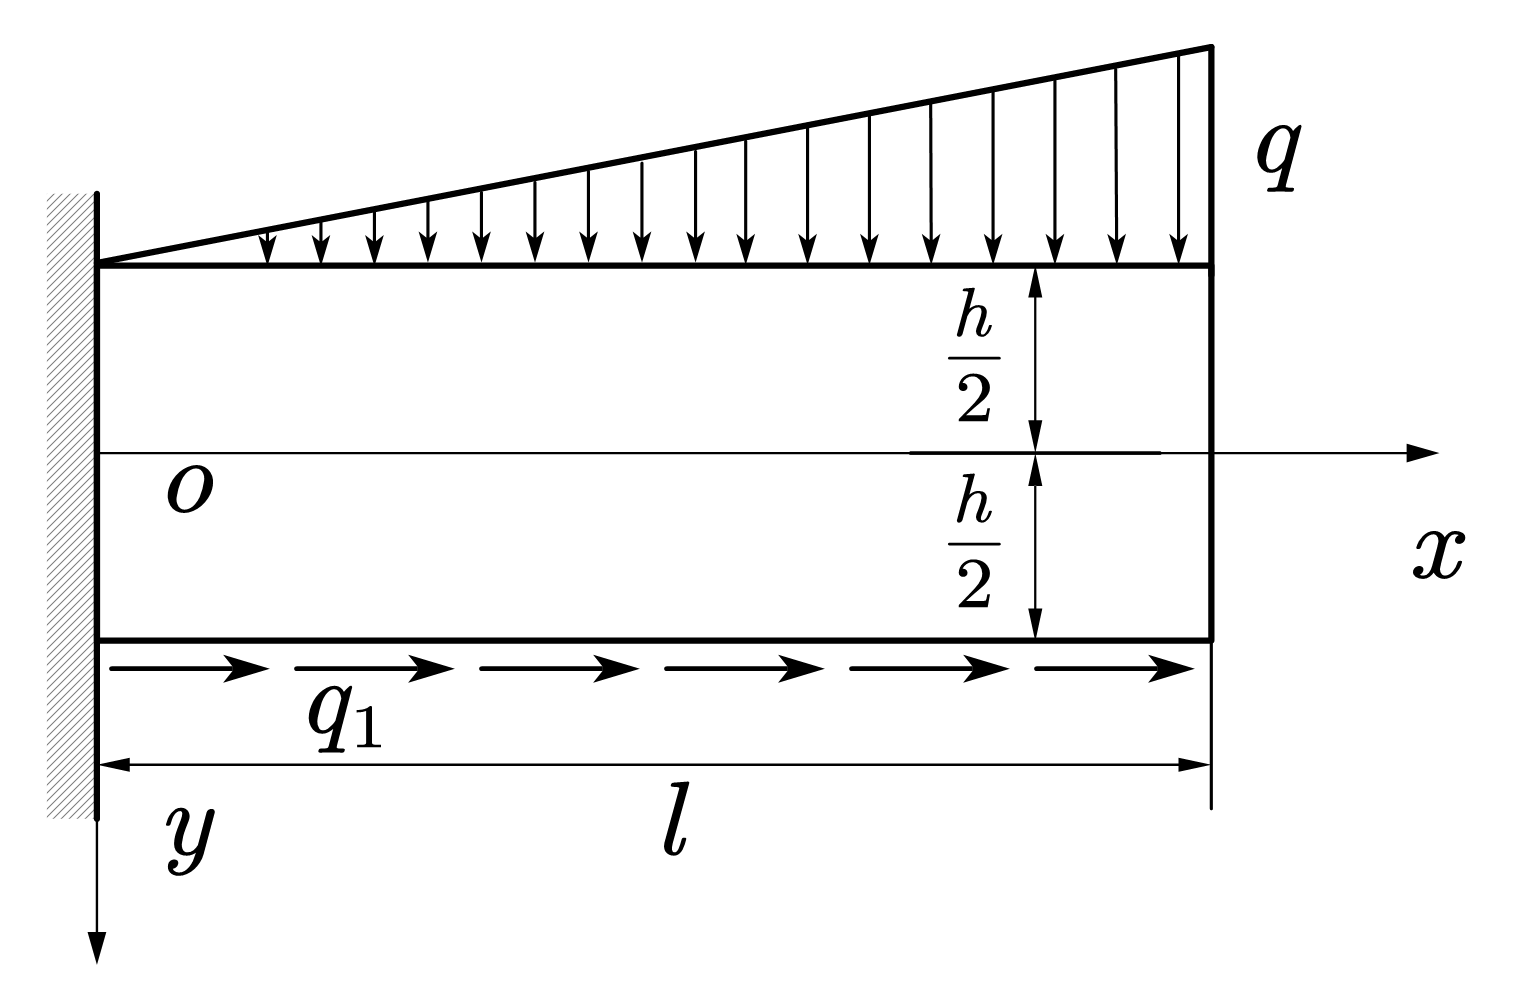
\includegraphics[scale=0.45]{figure/2-1.png}}
\begin{remark}
	\quad\\
	左:\[\left( u \right) _{x=0}=0,\left( v \right) _{x=0}=0\]
	右:\[\left( \sigma _x \right) _{x=l}=0,\left( \tau _{xy} \right) _{x=l}=0\]
	下:\[\left( \sigma _y \right) _{y=\frac{h}{2}}=0,\left( \tau _{yx} \right) _{y=\frac{h}{2}}=q_1\]
	上:\[\left( \sigma _y \right) _{y=\frac{h}{2}}=-q\frac{x}{l},\left( \tau _{xy} \right) _{y=-\frac{h}{2}}=0\]
\end{remark}
\begin{example}
\end{example}
	\centerline{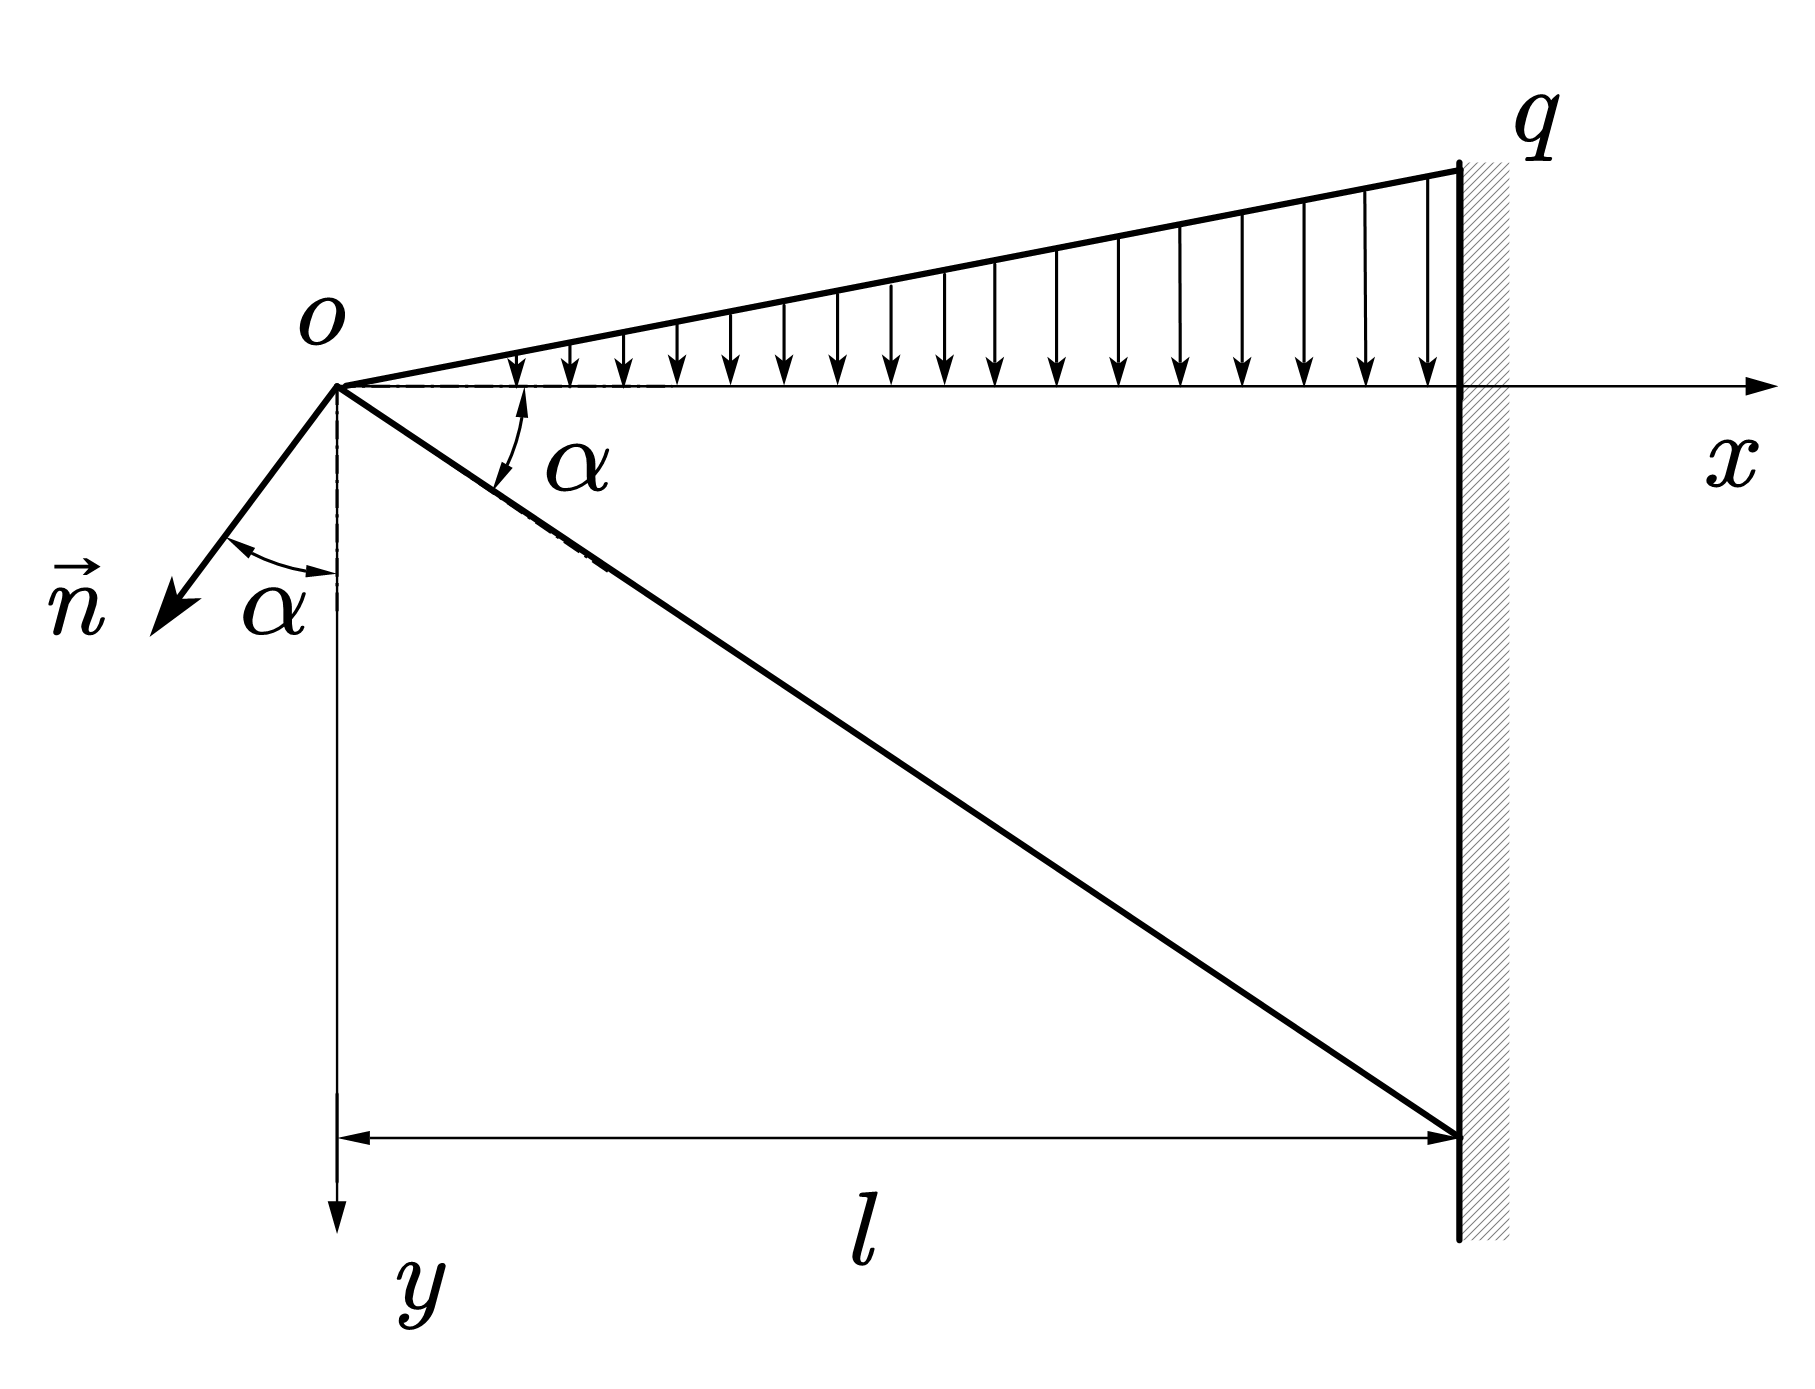
\includegraphics[scale=0.4]{figure/2-2.png}}
\begin{remark}
	\quad\\
	$y=0$的边界上:$\left( \sigma _y \right) _{y=0}=-q\frac{x}{l},\left( \tau _{xy} \right) _{y=0}=0$\\
	$x=l$边界上:$\left( u \right) _{x=l}=0,\left( v \right) _{x=l}=0$\\
	$y=x\tan \alpha$上:$l=\cos \left< \vec{n},\vec{x} \right> =\cos \left( \frac{\pi}{2}+\alpha \right) =-\sin \alpha ,m=\cos \alpha $
	\[\begin{cases}
	-\sin \alpha \sigma _x+\cos \alpha \tau _{yx}=0\\
	\cos \alpha \sigma _y-\sin \alpha \tau _{xy}=0\\
	\end{cases}\]
\end{remark}
\begin{example}
		水坝,左水右空
\end{example}
\centerline{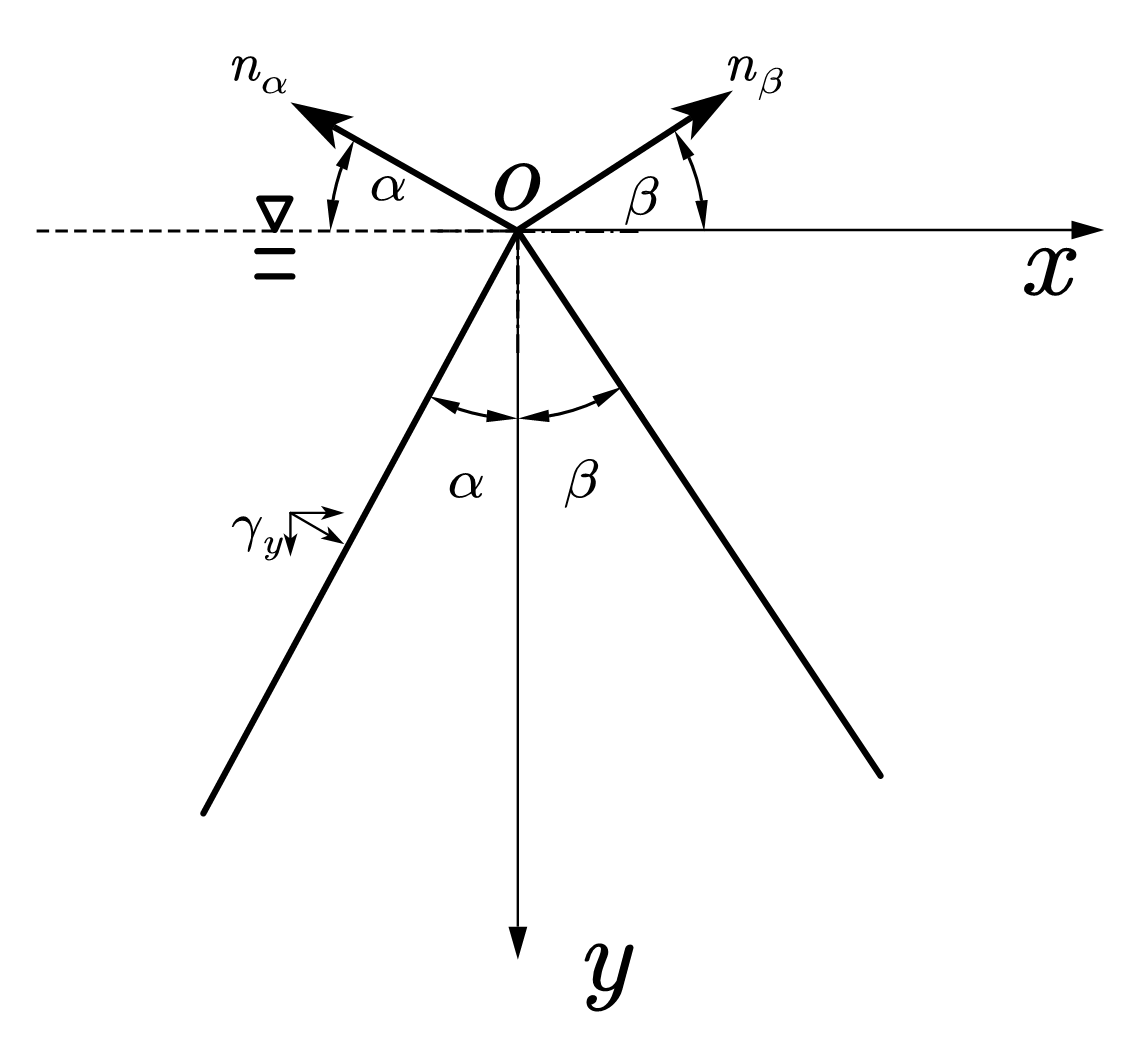
\includegraphics[scale=0.6]{figure/2-3.png}}
\begin{remark}
	\quad\\
	右侧:$l=\cos \beta ,m=\cos \left( \frac{\pi}{2}+\beta \right) =-\sin \beta $\[\begin{cases}
	\cos \beta \sigma _x-\sin \beta \tau _{xy}=0\\
	\cos \beta \tau _{xy}-\sin \beta \sigma _y=0\\
	\end{cases}\]
	左侧:$l=-\cos \alpha ,m=-\sin \alpha $\[\begin{cases}
	-\cos \alpha \sigma _x-\tau _{xy}\sin \alpha =\gamma y\cos \alpha\\
	-\cos \alpha \tau _{xy}-\sigma _y\sin \alpha =\gamma y\sin \alpha\\
	\end{cases}\]	
\end{remark}

\begin{example}
\end{example}
\centerline{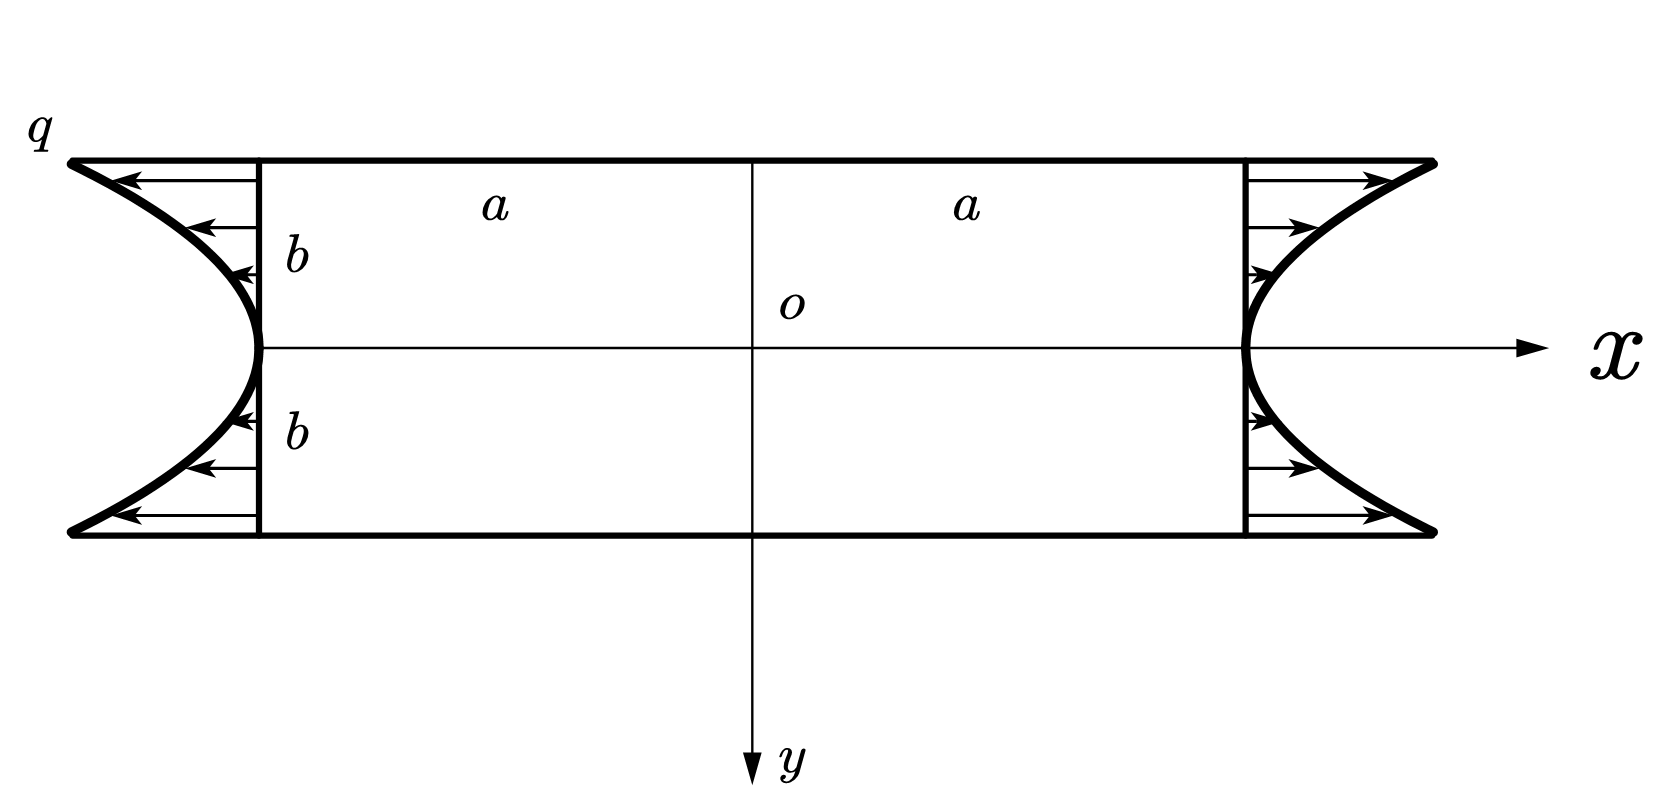
\includegraphics[scale=0.5]{figure/2-4.png}}
\begin{remark}
	上下:$\left( \sigma _y \right) _{y=\pm b}=0,\left( \tau _{xy} \right) _{y=\pm b}=0$\\
	左右:$\left( \sigma _x \right) _{x=\pm a}=q\left( \frac{y}{b} \right) ^2,\left( \tau _{xy} \right) _{x=\pm a}=0$
\end{remark}

\begin{example}
设有矩形截面的竖柱,密度为$\rho$,应力分量为$\begin{cases}
\sigma _x=0\\
\sigma _y=C_1y+C_2\\
\tau _{xy}=0\\
\end{cases}$试着分别利用$a$和$b$确定常数$C_1$和$C_2$。
\end{example}
\begin{center}
	\begin{minipage}[c]{0.3\textwidth}
		\centering
		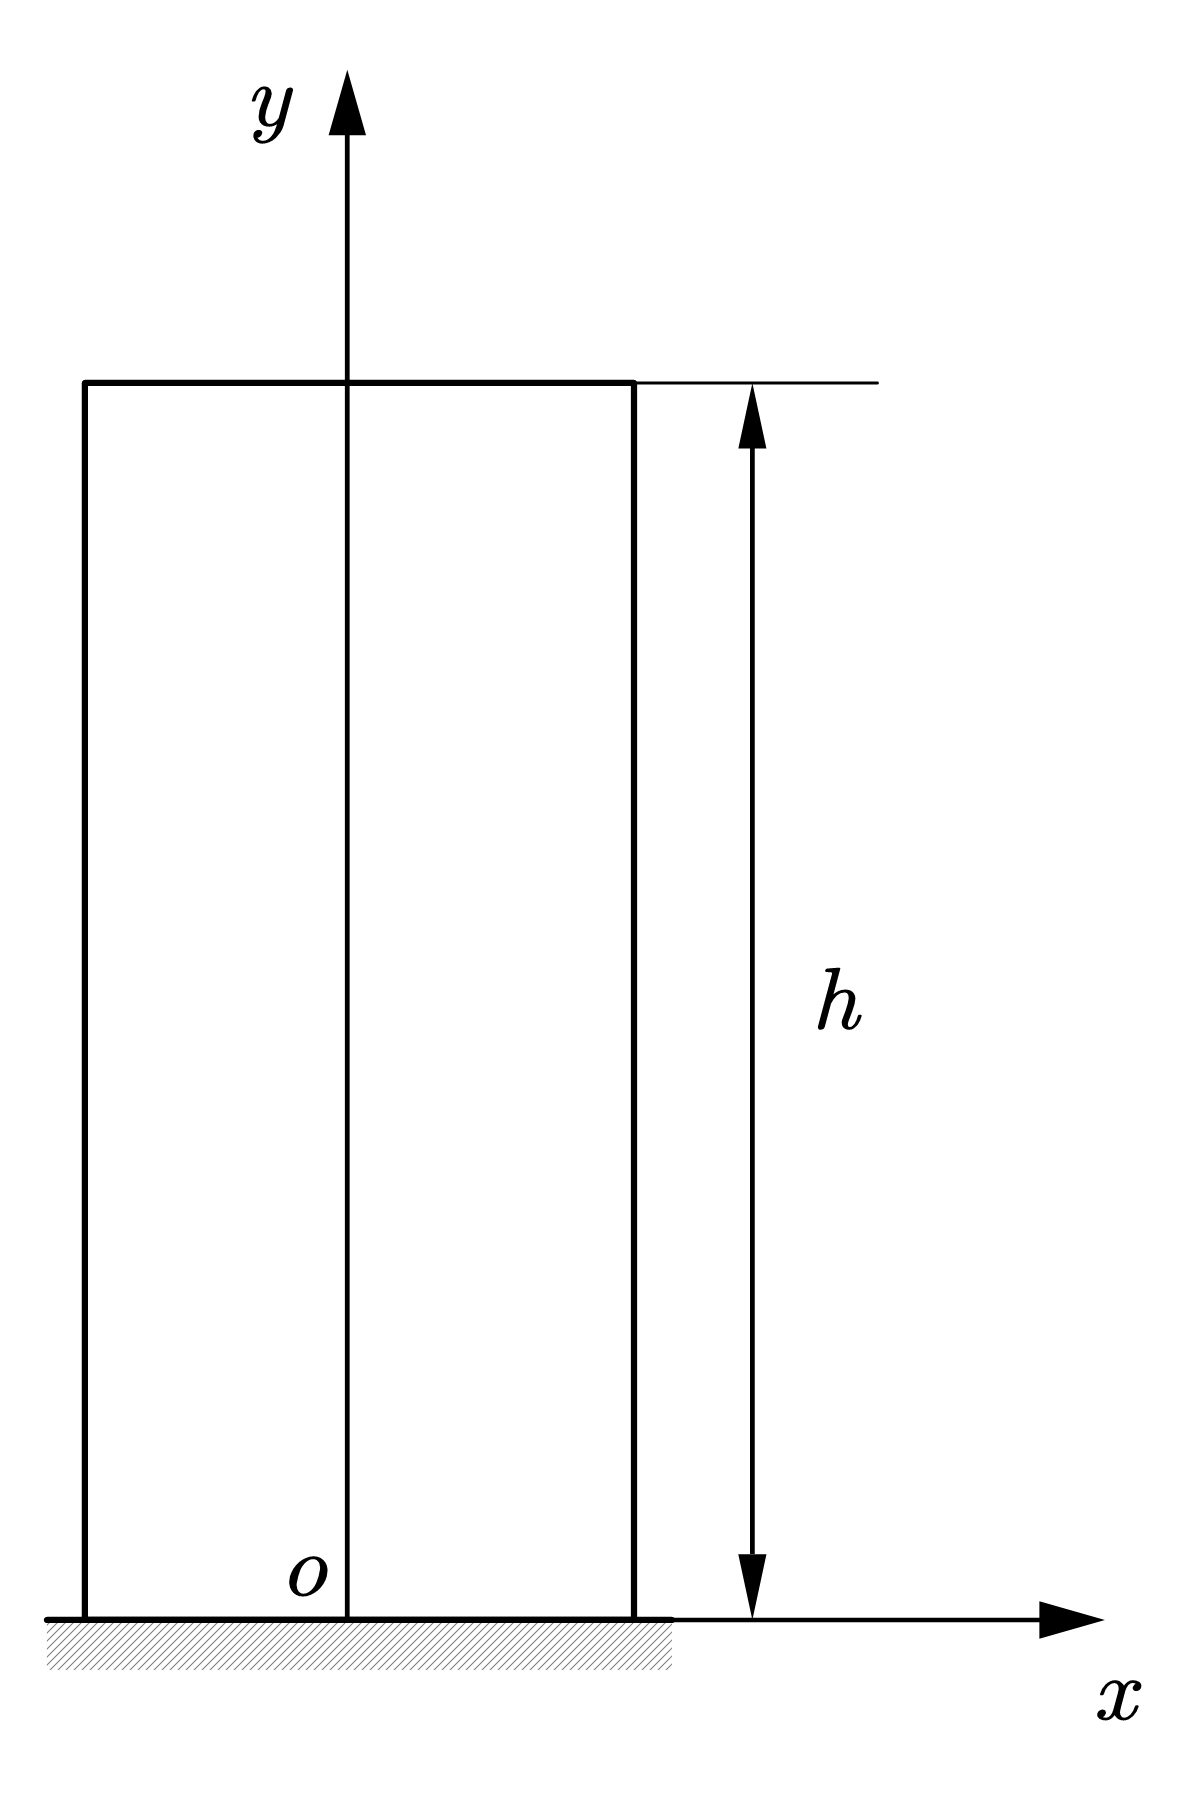
\includegraphics[scale=0.3]{figure/2-5.png}\\
		$a$\\
		\begin{flushleft}
			上:$\left( \sigma _y \right) _{y=h}=0$\\
		下:$\left( \sigma _y \right) _{y=0}=-\rho gh$\\
		则:\[\begin{cases}
		C_1=\rho g\\
		C_2=-\rho gh\\
		\end{cases}\]
		\end{flushleft}
	\end{minipage}
\begin{minipage}[c]{0.3\textwidth}
	\centering
	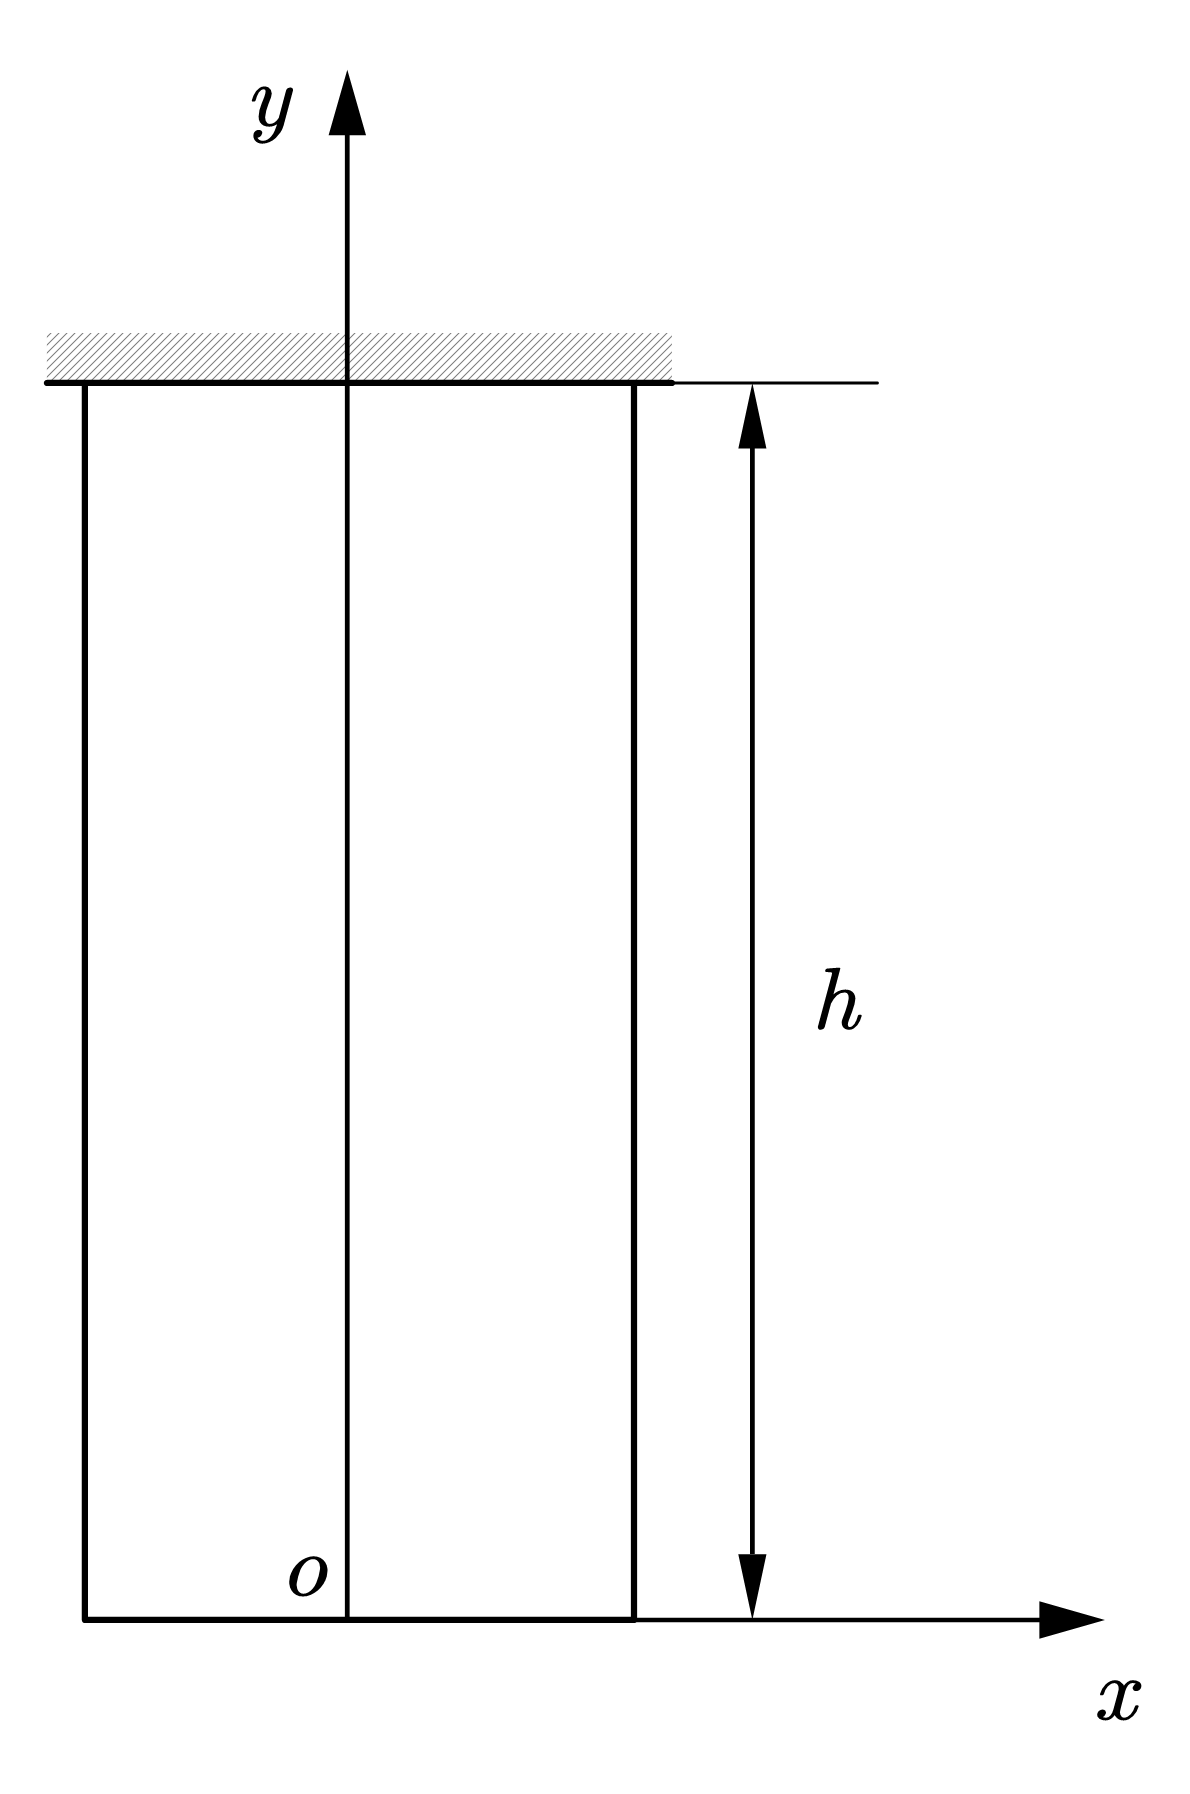
\includegraphics[scale=0.3]{figure/2-6.png}\\
	$b$\\
	\begin{flushleft}
		上:$\left( \sigma _y \right) _{y=h}=-\rho gh$\\
	下:$\left( \sigma _y \right) _{y=0}=0$\\
	则:\[\begin{cases}
	C_1=-\rho g\\
	C_2=0\\
	\end{cases}\]
	\end{flushleft}
\end{minipage}
\end{center}

\begin{example}
	证明$A$处无应力存在。
\end{example}
\centerline{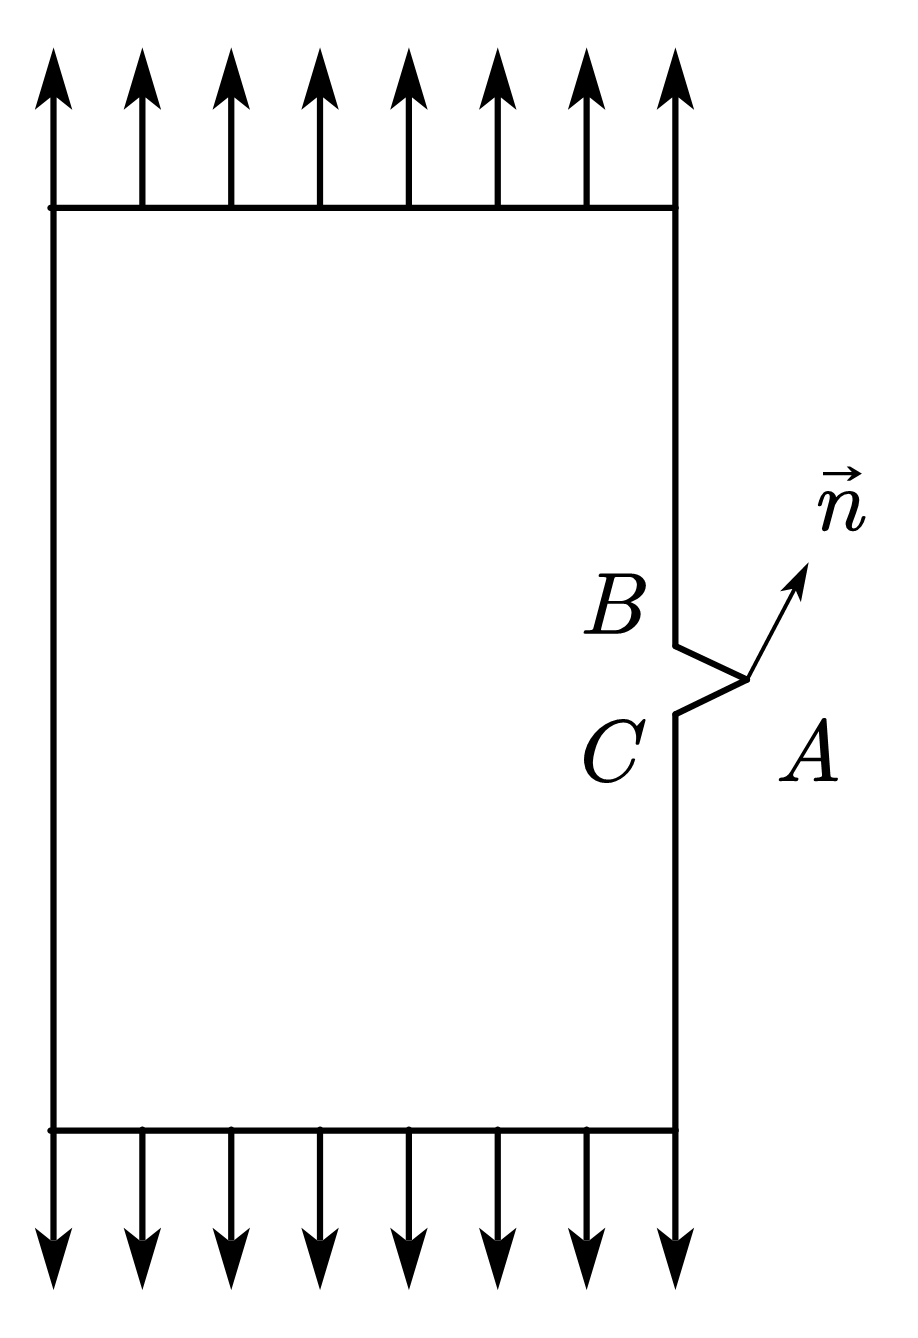
\includegraphics[scale=0.4]{figure/2-7.png}}
\begin{proof}
	边界条件:\[\begin{cases}
	l\sigma _x+m\tau _{xy}=0\\
	l\tau _{xy}+m\sigma _y=0\\
	\end{cases}\]
	$l,m$是任意系数,则矩阵$\left[ \begin{matrix}
	\sigma _x&		\tau _{xy}\\
	\tau _{yx}&		\sigma _y\\
	\end{matrix} \right] $为零矩阵,即$A$处无应力。
\end{proof}
\begin{example}
	考虑两端固定的一维杆件,只受重力作用,$f_x=0,f_y=\rho g$使用位移法求解。
\end{example}
\centerline{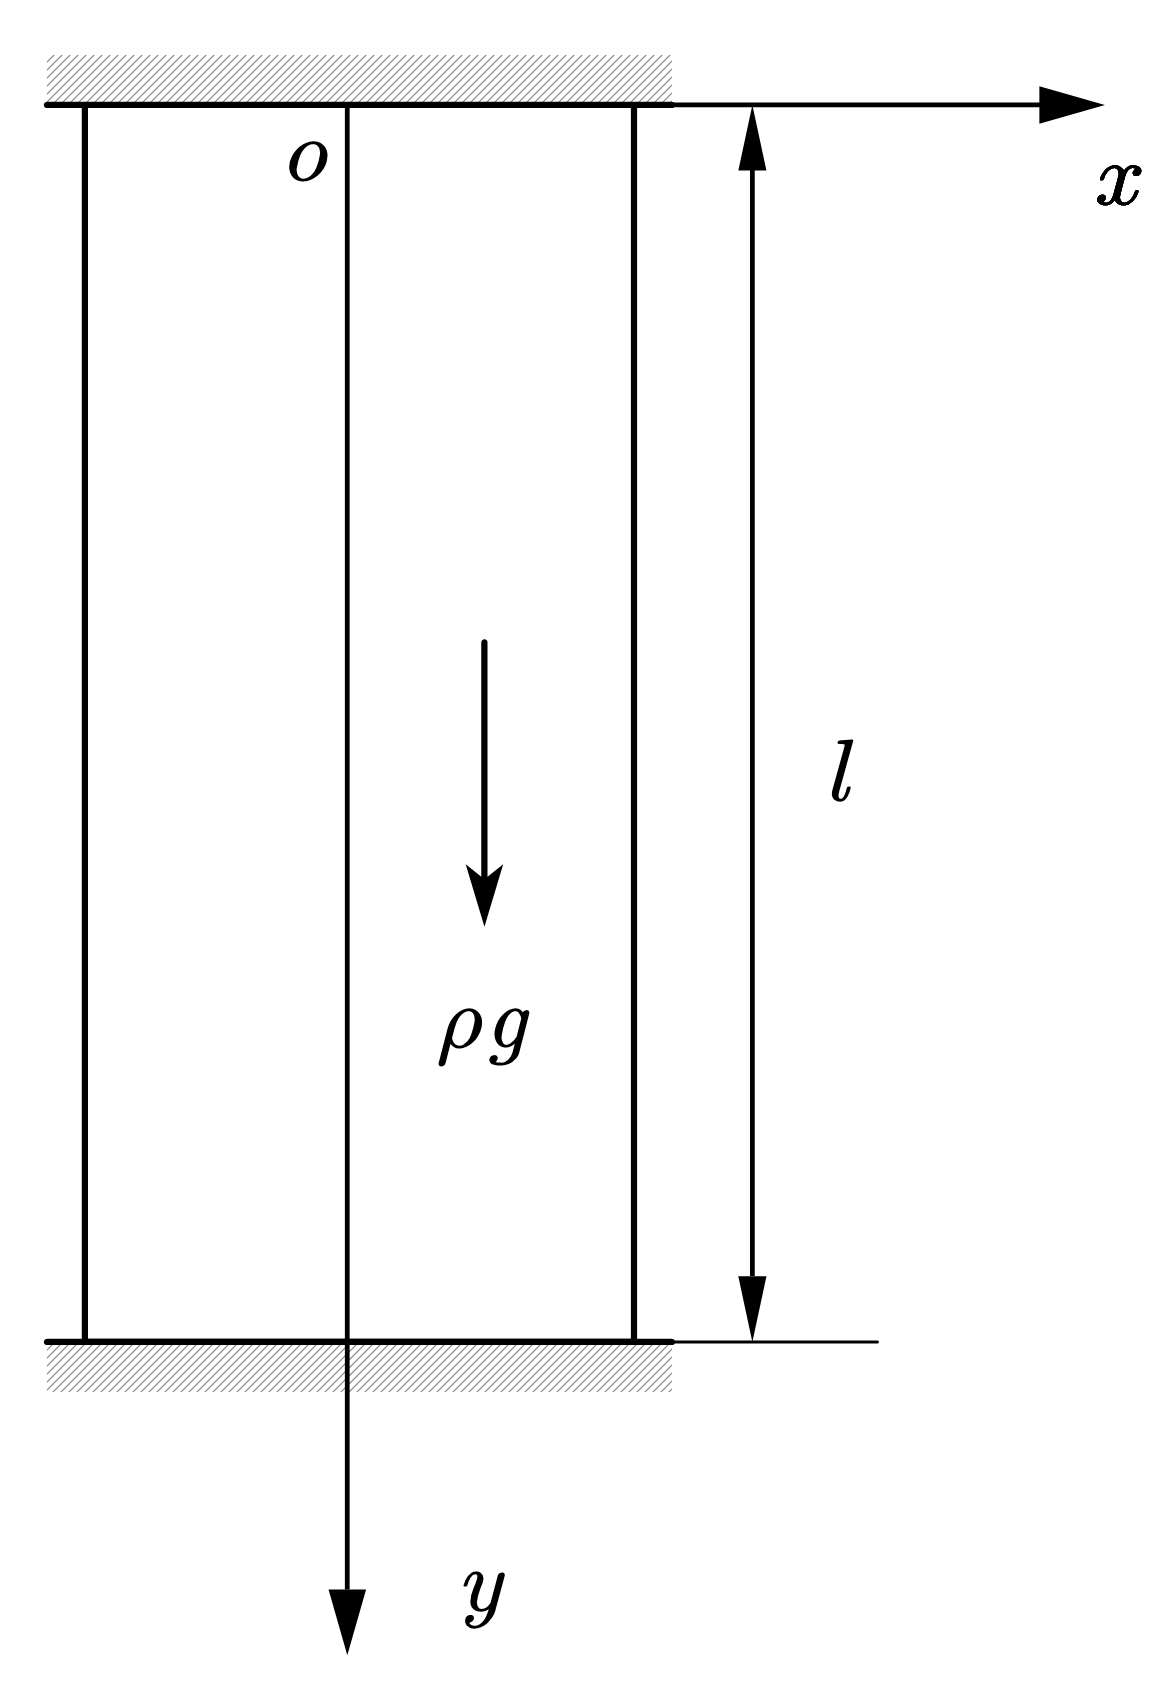
\includegraphics[scale=0.4]{figure/2-8.png}}
\begin{example}
	考虑一端固定的一维杆件,只受重力作用,$f_x=0,f_y=\rho g$使用位移法求解。
\end{example}
\centerline{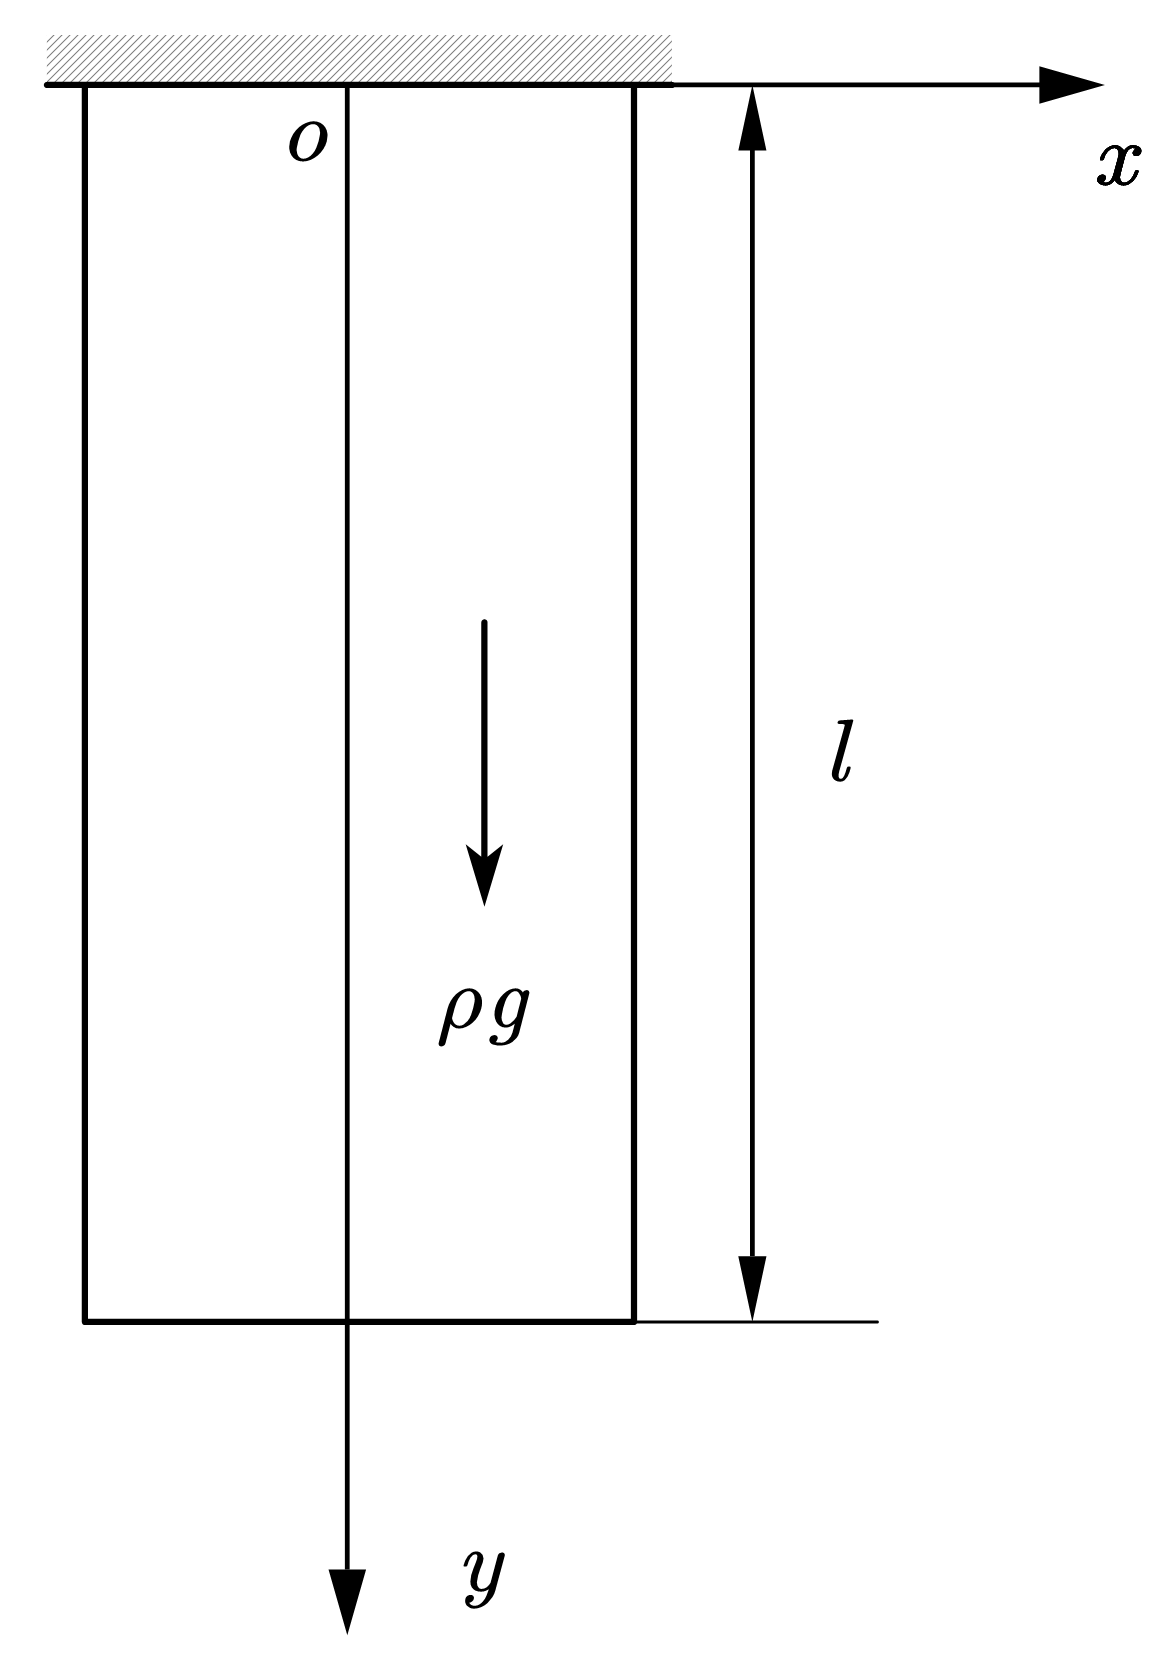
\includegraphics[scale=0.4]{figure/2-9.png}}

\begin{example}
	若$\varepsilon _x=ay^2,\varepsilon _y=bx^2,\gamma _{xy}=\left( a+b \right) xy$是否可能成为弹性体的应变。
\end{example}
\begin{remark}
	
\end{remark}
\begin{example}
若$f_x=f_y=0,\sigma _x=ax^2,\sigma _y=by^2,\tau _{xy}=0$是否可能成为弹性体的应力?
\end{example}
\begin{remark}
	
\end{remark}

\begin{example}
	试列出图中的边界条件
\end{example}
\centerline{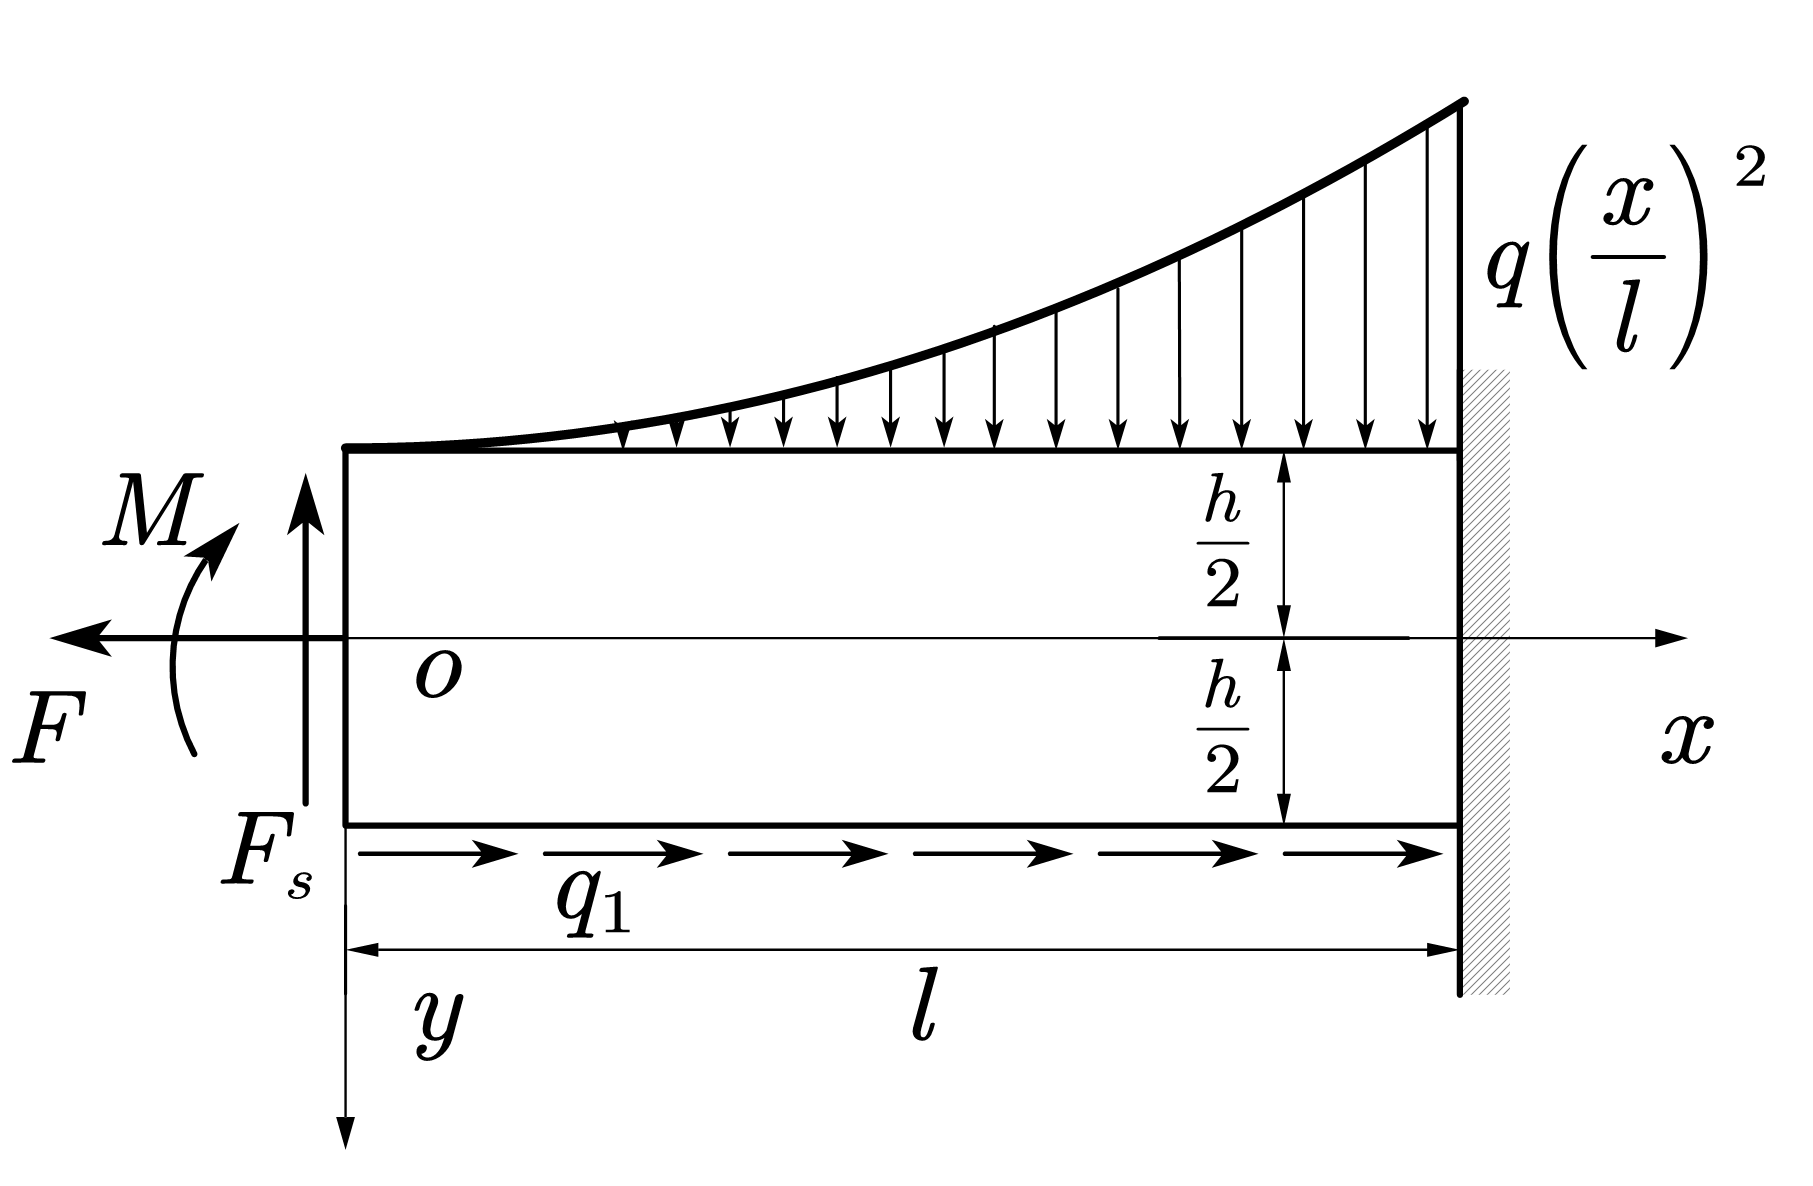
\includegraphics[scale=0.5]{figure/2-10.png}}

\begin{example}
	试列出图中的边界条件
\end{example}
\centerline{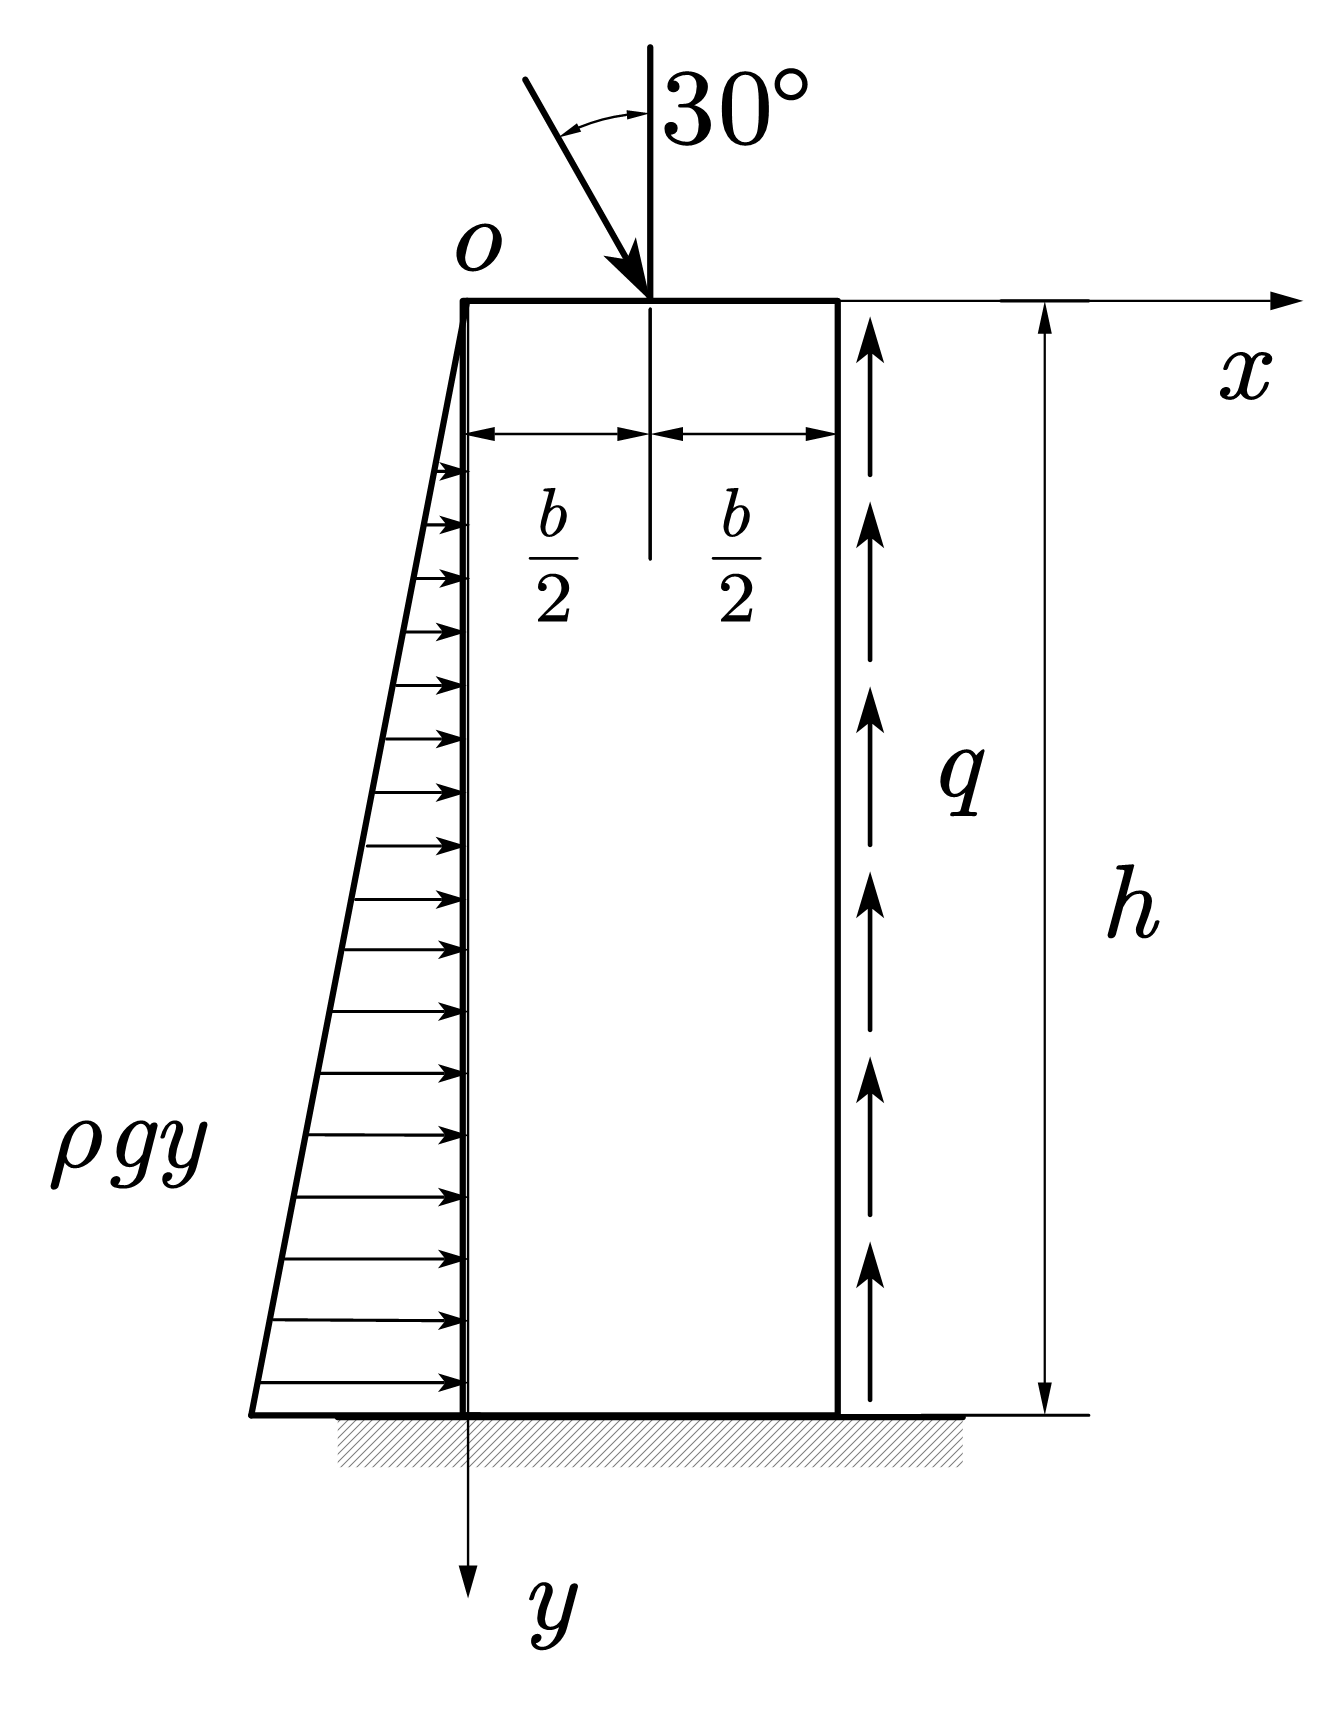
\includegraphics[scale=0.5]{figure/2-11.png}}

\begin{example}
	\quad
	\begin{enumerate}
		\item $\sigma _x=Ax+By,\sigma _y=Cx+Dy,\tau _{xy}=Ex+Fy$
		\item $\sigma _x=A\left( x^2+y^2 \right) ,\sigma _y=B\left( x^2+y^2 \right) ,\tau _{xy}=Cxy$
	\end{enumerate}
\end{example}

\begin{example}
	试验证下列应力分量是否是图示问题的解答\[\sigma _x=\frac{y^2}{b^2}q,\sigma _y=0,\tau _{xy}=0\]
\end{example}
\centerline{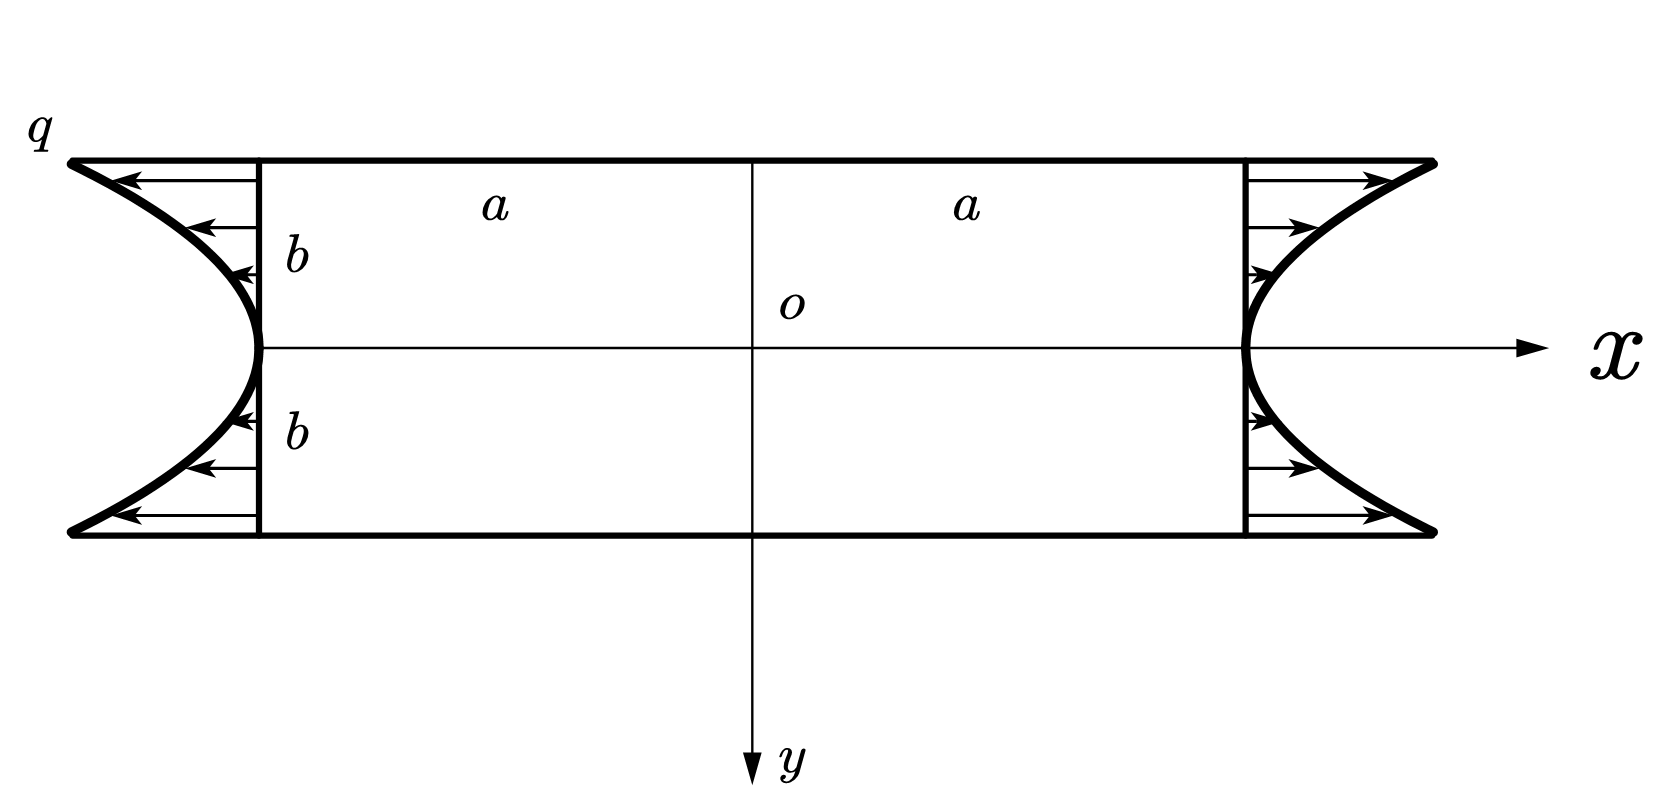
\includegraphics[scale=0.5]{figure/2-4.png}}

\begin{example}
	设有矩形截面悬臂梁,在自由端受集中力$F$作用,体力不计。试根据材料力学公式写出弯曲应力$\sigma _x$和切应力$\tau _{xy}$的表达式,然后证明这些表达试满足平衡方程和相容方程。再说明这些表达式是否是正确的解答。
\end{example}
\centerline{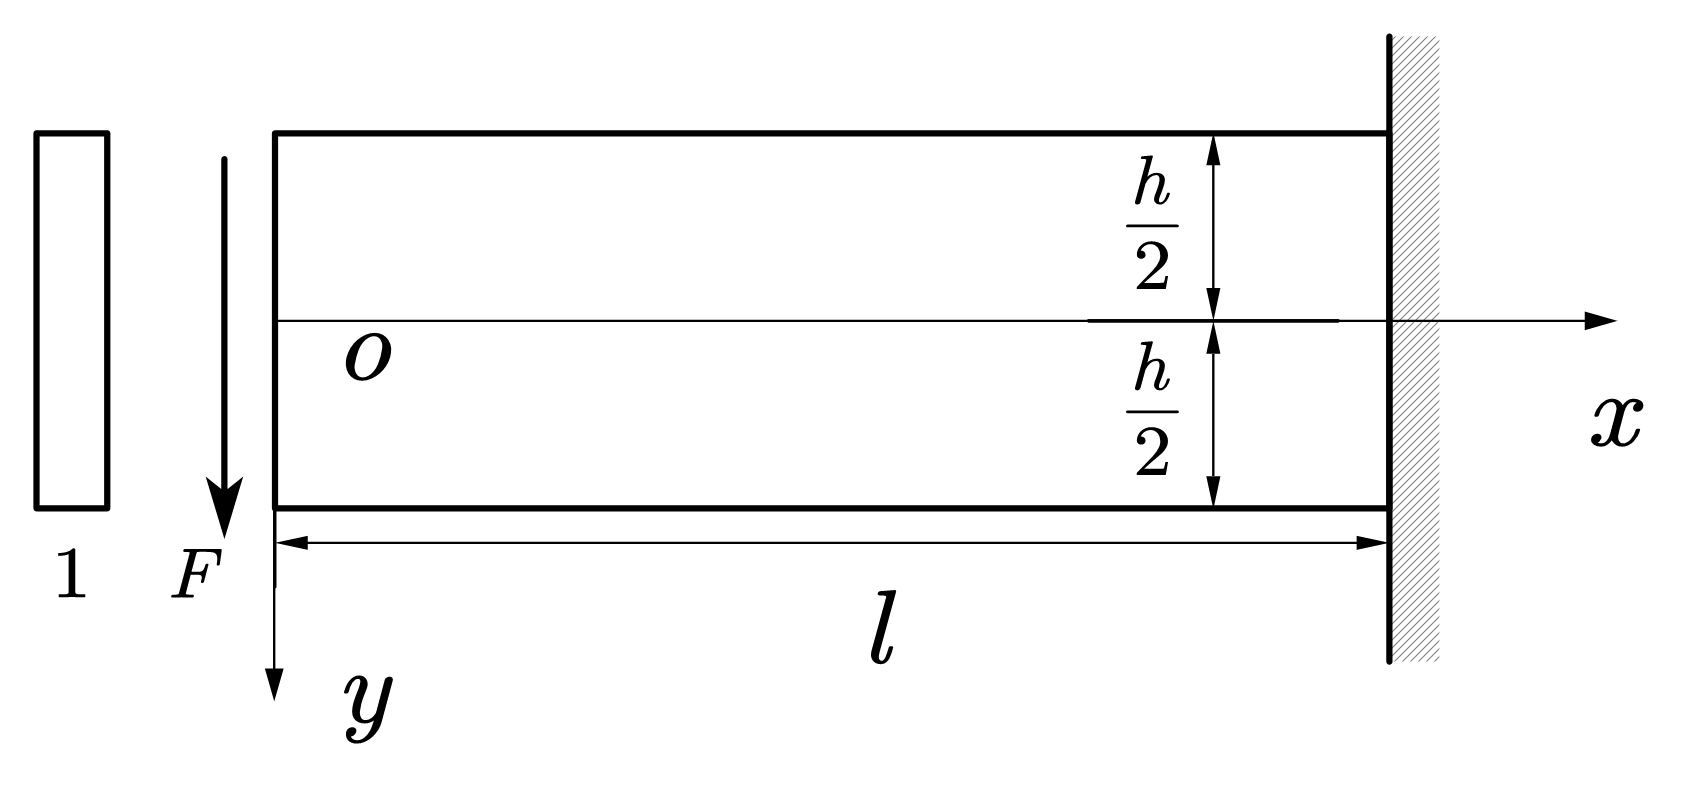
\includegraphics[scale=0.5]{figure/2-12.png}}

\begin{example}
	试用下列应力表达式求解其应力\[\begin{cases}
	\sigma _x=-\frac{q}{h^3}\left( 6x^2y-4y^3 \right)\\
	\sigma _y=-\frac{2q}{h^3}y^3-C_1y+C_2\\
	\tau _{xy}=\frac{6qxy^2}{h^3}+C_1x\\
	\end{cases}\]
\end{example}
\centerline{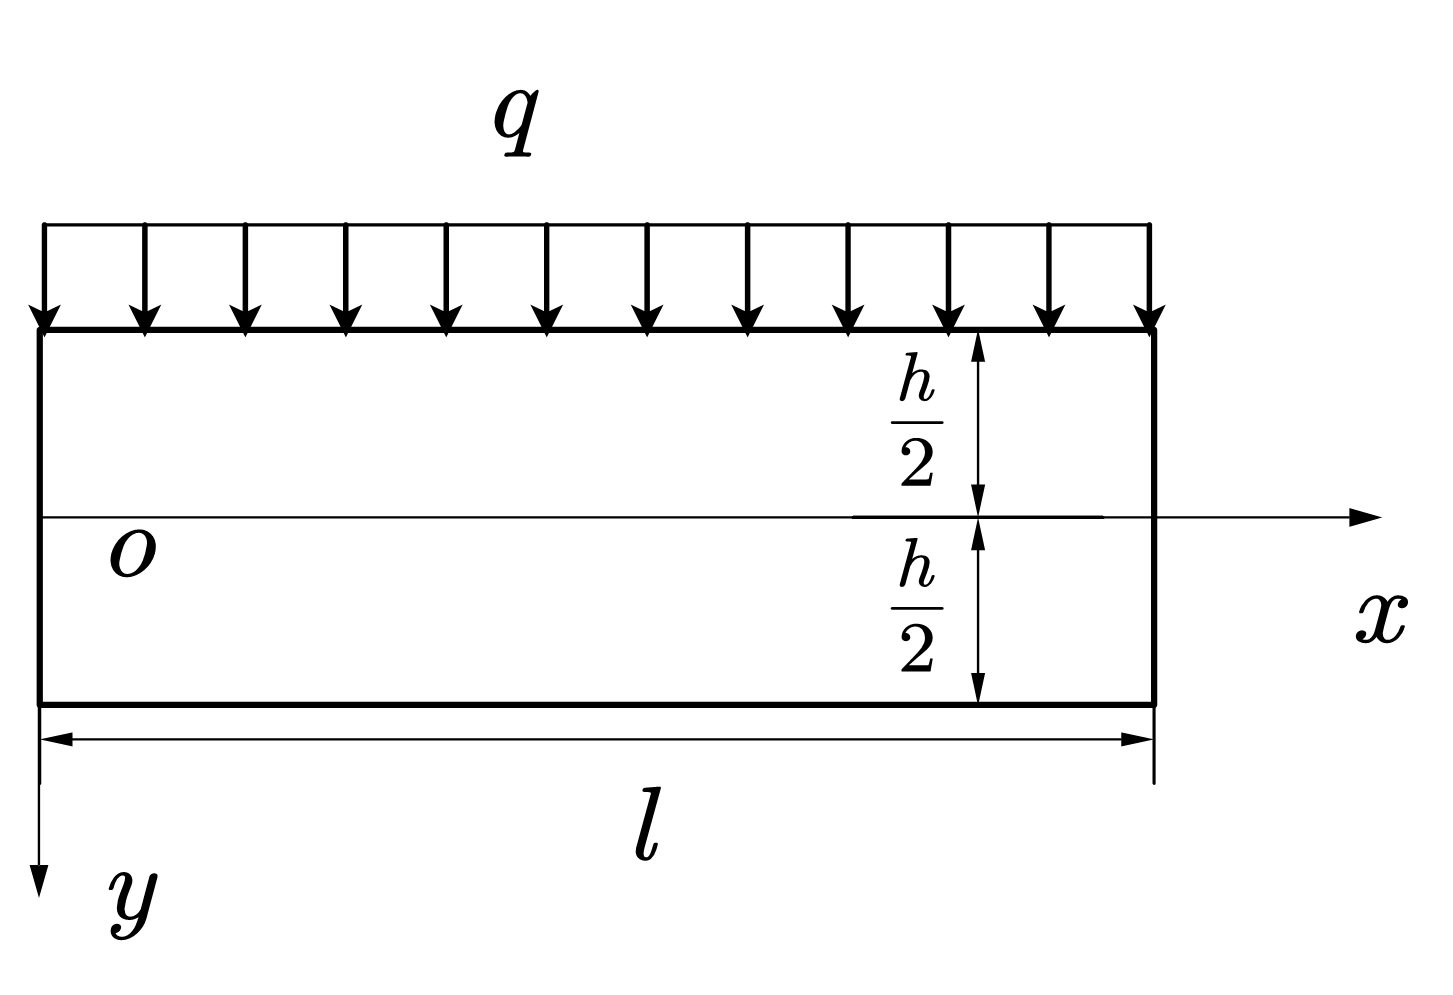
\includegraphics[scale=0.5]{figure/2-13.png}}

\begin{example}
	在材料力学中,当矩形截面梁(厚度$\delta =1$),受任意的横向荷载$q\left( x \right) $作用而弯曲,弯曲应力公式为$\sigma _x=\frac{M\left( x \right)}{I}y$。\\
	试由平衡微分方程导出切应力和挤压应力$\sigma _y$的公式。
\end{example}
\centerline{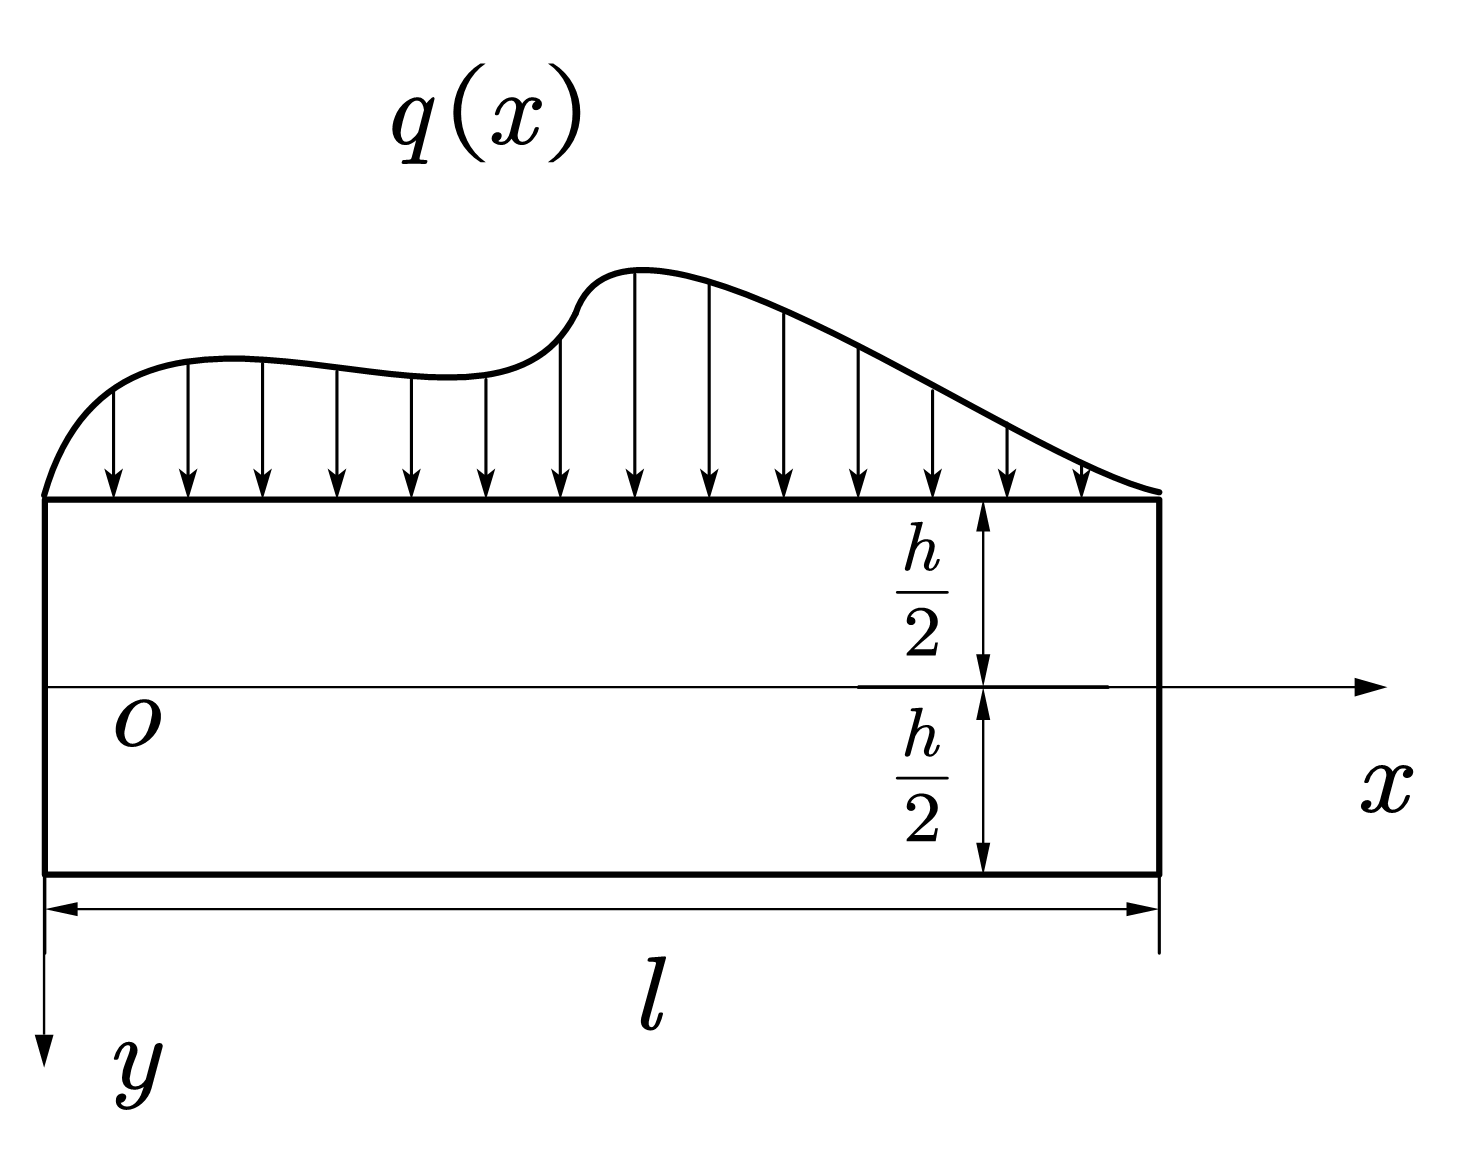
\includegraphics[scale=0.5]{figure/2-14.png}}